%-----------------------------------------------------------------------------
% cabeçalho
%-----------------------------------------------------------------------------
\documentclass{beamer}

% para criar um documento para acompanhamento, comente a linha acima e
% descomente as linhas abaixo.
%\documentclass[handout]{beamer}
%\usepackage{pgfpages}
%\pgfpagesuselayout{4 on 1}[a4paper,border shrink=5mm]


% localização
\usepackage[utf8x]{inputenc}
\usepackage[brazil]{babel}
%\usepackage{abntex}

% embelezamento
\usepackage{amssymb,amsmath,amsfonts}
\numberwithin{equation}{section}
\usepackage{enumerate}
\usepackage{xspace}
%\usetheme{Goettingen} % <---- so com crane
%\usetheme{sidebar}   % <---- com crane fica bom
%\usecolortheme{crane} % <---- Goettingen com crane
\usepackage{colortbl}
\usepackage{url}
\usepackage{color}
\usepackage{listings}             % Include the listings-package


% figuras
\usepackage{tikz}
\usetikzlibrary{arrows}

% Sumário no início de cada seção
\AtBeginSection[]
{
  \begin{frame}<beamer>{Estrutura da apresentação}
    \tableofcontents[currentsection]
  \end{frame}
}

% comandos
\definecolor{meuvermelho}{RGB}{200,40,40}
\definecolor{meuazul}{RGB}{40,40,140}
\newcommand{\enfase}[1]{{\color{meuvermelho}#1}}
\newcommand{\enfasel}[1]{{\color{meuazul}#1}}
\newcommand{\inlet}{\emph{inlet}}
\newcommand{\inlets}{\emph{inlets}}
\newcommand{\outlet}{\emph{outlet}}
\newcommand{\outlets}{\emph{outlets}}
\newcommand{\Inlet}{\emph{Inlet}}
\newcommand{\Inlets}{\emph{Inlets}}
\newcommand{\Outlet}{\emph{Outlet}}
\newcommand{\Outlets}{\emph{Outlets}}
\newcommand{\external}{\emph{external}\xspace}
\newcommand{\externals}{\emph{\enfase{externals}}\xspace}
\newcommand{\External}{\emph{External}\xspace}
\newcommand{\Externals}{\emph{Externals}\xspace}


%-----------------------------------------------------------------------------
% Dados para o primeiro slide
%-----------------------------------------------------------------------------

\title
{Como estender o Pure Data através de \emph{externals} em C}

%\subtitle
%{}

\author
{Flávio Luiz Schiavoni\\
\footnotesize{fls@ime.usp.br}}

\institute
[Universidade de São Paulo]
{
  Departamento de Ciência da Computação\\
  Instituto de Matemática e Estatística \\
  Universidade de São Paulo
}

\date{\today}


\lstset{ %
language=C,                % the language of the code
basicstyle=\footnotesize\ttfamily,       % the size of the fonts that are used for the code
%basicstyle=\footnotesize,       % the size of the fonts that are used for the code
numbers=left,                   % where to put the line-numbers
numberstyle=\tiny,      % the size of the fonts that are used for the line-numbers
%stepnumber=2,                   % the step between two line-numbers. If it's 1, each line 
                                % will be numbered
numbersep=8pt,                  % how far the line-numbers are from the code
backgroundcolor=\color{white},  % choose the background color. You must add \usepackage{color}
showspaces=false,               % show spaces adding particular underscores
showstringspaces=false,         % underline spaces within strings
showtabs=false,                 % show tabs within strings adding particular underscores
frame=single,                   % adds a frame around the code
tabsize=2,                      % sets default tabsize to 2 spaces
captionpos=b,                   % sets the caption-position to bottom
breaklines=true,                % sets automatic line breaking
breakatwhitespace=true,
breakatwhitespace=true,        % sets if automatic breaks should only happen at whitespace
title=\lstname,                 % show the filename of files included with \lstinputlisting;
                                % also try caption instead of title
escapeinside={\%*}{*)},         % if you want to add a comment within your code
%xleftmargin={2em},
%xrightmargin={2em},
columns=fixed,
emptylines=*1,
firstnumber=auto,
morekeywords={*,...}            % if you want to add more keywords to the set
}

% Caminho para imagens
\graphicspath{{./../images/}}


%-----------------------------------------------------------------------------
% Documento
%-----------------------------------------------------------------------------
\begin{document}

\begin{frame}
  \titlepage
\end{frame}

%-----------------------------------------------------------------------------
\begin{frame}{Objetivo da apresentação}

Introduzir à escrita de \emph{externals} para Pure Data, considerando:
\begin{itemize}
  \item Como escrever.
  \item Como compilar.
  \item Exemplos.
\end{itemize}
\end{frame}

%-----------------------------------------------------------------------------
\begin{frame}{Estrutura da apresentação}
  \tableofcontents
\end{frame}

% Since this a solution template for a generic talk, very little can
% be said about how it should be structured. However, the talk length
% of between 15min and 45min and the theme suggest that you stick to
% the following rules:  

% - Exactly two or three sections (other than the summary).
% - At *most* three subsections per section.
% - Talk about 30s to 2min per frame. So there should be between about
%   15 and 30 frames, all told.

%-----------------------------------------------------------------------------
% Seções
%-----------------------------------------------------------------------------
\section{Introdução}

\begin{frame}{Pure Data}
\begin{figure}
\centering
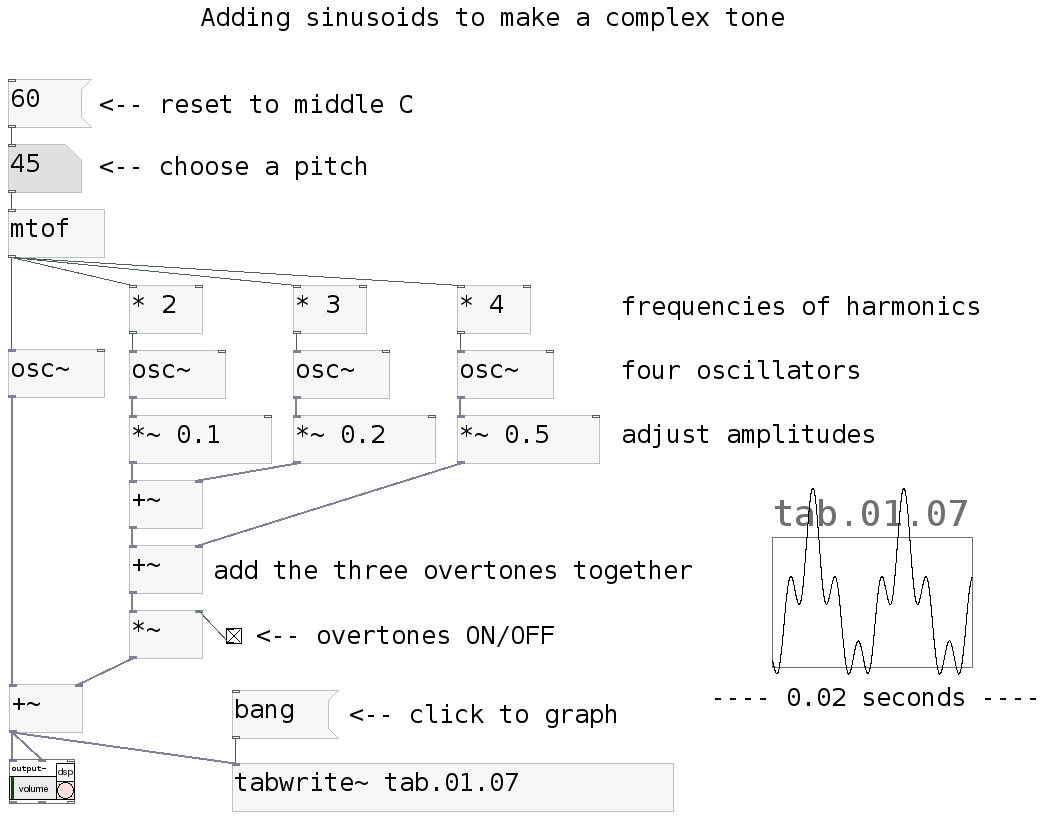
\includegraphics[width=0.7\textwidth]{../images/pd-facil}
\end{figure}
\end{frame}


\begin{frame}{Formas de estender o Pure Data}
Existem algumas formas de estender as funcionalidades do Pure Data:
\begin{itemize}
\item Subpatches.
\item \enfasel{Externals}.
\item Alterações no código-fonte.
\end{itemize}
\pause
\vspace{1em}
Este seminário trata da extensão do Pure Data através da criação de
\externals em C.
\end{frame}


\begin{frame}[fragile]{Organização do código-fonte}
Algumas informações sobre o código do Pure Data:
\begin{itemize}
\item Publicado sob a licença \enfasel{Standard Improved BSD License}.
\item Organizado de forma orientada a objetos.
\begin{itemize}
\item Classes são tipos.
\item Objetos (gráficos) do Pure Data são instâncias de classes.
dados e assinaturas de funções: \texttt{m\_pd.h}.
\end{itemize}
\item Existe um arquivo de cabeçalho com constantes, tipos, estruturas de
dados e assinaturas de funções: \texttt{m\_pd.h}.
\end{itemize}
\end{frame}


\begin{frame}[fragile]{Compilação}
\begin{lstlisting}
EXTNAME=meu_external
cc -DPD -fPIC -Wall -o ${EXTNAME}.o -c ${EXTNAME}.c
ld -shared -lc -lm -o ${EXTNAME}.pd_linux ${EXTNAME}.o
rm ${EXTNAME}.o
\end{lstlisting}
O Pure Data procura por objetos com nomes diferentes em cada sistema:
\begin{itemize}
  \item \texttt{meu\_external.\enfase{pd\_linux}} (GNU/Linux).
  \item \texttt{meu\_external.\enfase{pd\_irix5}} (Irix 5).
  \item \texttt{meu\_external.\enfase{pd\_darwin}} (Mac OS X).
  \item \texttt{meu\_external.\enfase{dll}} (MS Windows).
\end{itemize}
\end{frame}


\begin{frame}[fragile]{Arquivos de ajuda}
Um arquivo de ajuda é um patch do Pure Data com:
\begin{itemize}
\item Um nome informativo: \texttt{meu\_external\enfase{-help}.pd}.
\item Instruções de uso.
\item Exemplos de utilização.
\end{itemize}
\vspace{2em}
A seguinte função associa um arquivo de ajuda a uma classe de \external:
\begin{lstlisting}
class_sethelpsymbol(meu_external_class, gensym("meu_external_class-help"));
\end{lstlisting}
\end{frame}


\begin{frame}{Utilizando \externals}
Passos para utilizar um \external no Pure Data:
\begin{enumerate}
\item Escreva um arquivo \texttt{.c} com as funções, classes e métodos.
\item Compile o código-fonte para criar uma biblioteca compartilhada.
\item Informe ao Pure Data o caminho para o \external através de uma das
opções abaixo:
  \begin{itemize}
    \item Na criação do objeto, insira o caminho completo (relativo ou
    absoluto) para o objeto do \external.
    \item Na linha de comando, utilize a opção \enfasel{\texttt{-path
    <caminho>}}.
    \item Na interface gráfica, acesse a opção \enfasel{\texttt{File} $\rightarrow$
    \texttt{Path...}}.
  \end{itemize}
\item Crie um objeto na interface gráfica do Pd com o nome do arquivo do \external, sem a extensão.
\end{enumerate}
\end{frame}


\begin{frame}{Utilizando \externals}
\begin{figure}[h!]
  \centering
  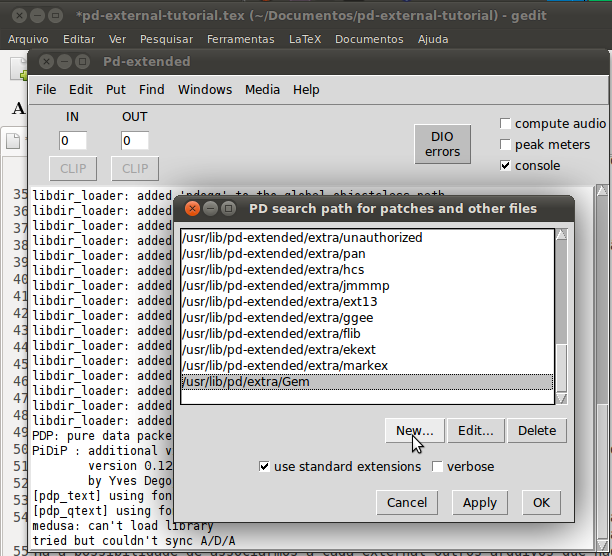
\includegraphics[width=0.7\textwidth]{../images/path}
  \caption{Adicionando o diretório de um \external ao caminho de busca do Pure Data.}
  \label{fig:search-path}
\end{figure}
\begin{itemize}
\item
\end{itemize}
\end{frame}

% ----------------------------------------------------------------------------
% O básico de um \external
% ----------------------------------------------------------------------------

\chapter{O básico de um \external}

Escrever um \external significa seguir as recomendações da API. Peço ao leitor
bastante paciência pois este tutorial pretende andar um pouco devagar para
mostrar os passos da escrita de um \external.

\section{Um \external simples}

Como dissemos anteriormente, a arquitetura do Pure Data é organizada de acordo
com o paradigma de orientação a objetos: cada objeto gráfico do Pure Data
corresponde a uma instância de uma classe. Neste sentido, um \external está
associado a uma estrutura de dados que representa uma classe em C. Para cada
classe é necessário haver métodos de instanciação, destruição, processamento
de sinais, tratamento de mensagens, etc.

A infraestrutura mínima para o funcionamento de uma classe consiste em uma
estrutura de dados para a representação da classe, que deve ser chamada
\texttt{t\_<external>}, e dois métodos obrigatórios: \texttt{<external>\_setup()}
e \texttt{<external>\_new()}. A convenção de nomes utilizada no Pure Data é de
que toda função deve ser nomeada da forma
\texttt{<external>\_<metodo>(<argumentos>)}.

A estutura de dados que representa uma classe do Pure Data deve
obrigatoriamente possuir o primeiro atributo do tipo \texttt{t\_object}, no
qual é armazenado o objeto instanciado no momento da instanciação.  Outros
atributos podem ser adicionados a esta estrutura de maneira que cada instância
da mesma classe possua os atributos necessários para seu funcionamento. Uma
classe que acessa um arquivo, por exemplo, pode possuir como atributos uma
string para guardar o caminho e um inteiro para guardar o descritor do
arquivo.

Um exemplo de estrutura de dados para representação de uma classe chamada
\texttt{example01} consiste no seguinte:

\vspace{1em}
\begin{lstlisting}
static t_class *example01_class;

typedef struct _example01 {
  t_object x_obj;
} t_example01;
\end{lstlisting}

Sempre que um \external é carregado pelo Pure Data, o método de nome
\texttt{<external>\_setup()} é executado. No exemplo dado acima, o Pure
Data irá procurar, no arquivo binário \texttt{example01.pd\_linux} que contém
a biblioteca compartilhada, o método de nome \texttt{example01\_setup(void)}.
Este método é utilizado para realizar a inicialização da classe, informando ao
Pure Data da existência de uma nova classe no sistema e associando a ela os
métodos de instanciação e destruição, além de outras informações:

\vspace{1em}
\begin{lstlisting}
void example1_setup(void) {
  example1_class = class_new(
    gensym("example1"),         // Nome simbolico
    (t_newmethod) example1_new, // Construtor
    0,                          // Destrutor
    sizeof (t_example1),        // Tamanho dos atributos
    CLASS_NOINLET,              // Flags da classe
    0                           // Tipos dos argumentos
  );
}
\end{lstlisting}

Dentro do método \texttt{<external>\_setup()} não há limite para o número de
classes a definir, de forma que é possível definir apenas uma classe (como no
exemplo 01) ou uma biblioteca inteira com várias classes (como no exemplo 03).
A introdução de uma nova classe no sistema é realizada pela função
\texttt{class\_new()}. São parâmetros da função \texttt{class\_new()}:

\begin{itemize}
\item Nome simbólico da classe.
\item Método construtor de um objeto.
\item Método destrutor de um objeto.
\item Tamanho do espaço de dados dos atributos de um objeto.
\item Flags que definem a representação gráfica do objeto.
\item Tipos dos parâmetros a serem passados para o construtor quando da
      instanciação de um objeto (veja o próximo capítulo).
\end{itemize}

É necessário terminar a lista de tipos de parâmetros com um número inteiro 0,
para indicar ao Pure Data que a lista de tipos terminou. Consulte a
documentação da função \texttt{class\_new()} para mais
detalhes\footnote{http://pdstatic.iem.at/externals-HOWTO/node9.html\#SECTION00092100000000000000}.

O método \texttt{<external>\_new()}, que foi associado como método de
instanciação de objetos na chamada de \texttt{class\_new()}, realiza a
instanciação de objetos propriamente dita. Neste método, além da instanciação
de um novo objeto através da função \texttt{pd\_new()}, é possível definir os
valores dos atributos da estrutura de dados da classe e também inicializar
quaisquer outros contextos que sejam necessários, como por exemplo abrir
arquivos, preencher vetores, alocar memória, etc.

\vspace{1em}
\begin{lstlisting}
// Construtor da classe
void * example01_new(void) {
    t_example1 *x = (t_example1 *) pd_new(example1_class);
    return (void *) x;
}
\end{lstlisting}

Após a criação da estrutura de dados dos métodos da forma mencionada acima, a
compilação realizada da forma descrita na seção \ref{sec:compiling}, e a
criação do objeto no Pure Data como descrito na seção \ref{sec:using}, o
resultado pode ser visto na figura \ref{fig:example01working}.

\begin{figure}[h!]
  \centering
  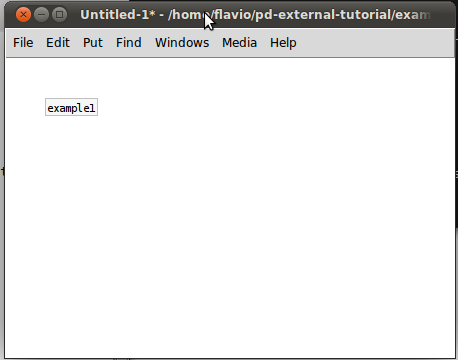
\includegraphics[width=0.7\textwidth]{example1}
  \caption{Nosso primeiro \external do PD. Ainda inútil. :-$\left.\right)$}
  \label{fig:example01working}
\end{figure}

\section{Uma biblioteca simples}

Um mesmo método \texttt{<external>\_setup()} pode definir várias classes
diferentes. A isto damos o nome de biblioteca. Para isto, o método
\texttt{<external>\_setup()} terá o mesmo nome do arquivo com a biblioteca mas
as classes  podem ter outros nomes. Veja o exemplo 03.

\vspace{1em}
\begin{lstlisting}
void example3_setup(void) {
    post("Initializing my library");

    myobj1_class = class_new(gensym("myobj1"),
            (t_newmethod) myobj1_new, // Constructor
            0,
            sizeof (t_myobj1),
	    CLASS_NOINLET,
            0);
    class_sethelpsymbol(myobj1_class, 
	gensym("myobj1-help"));

    myobj2_class = class_new(gensym("myobj2"),
            (t_newmethod) myobj2_new, // Constructor
            0,
            sizeof (t_myobj2),
	    CLASS_NOINLET,
            0);
    class_sethelpsymbol(myobj2_class, 
	gensym("myobj2-help"));

}
\end{lstlisting}

Se o arquivo foi feito corretamente, compilado corretamente e adicionado ao
caminho do PureData, teremos o resultado.

\begin{figure}[h!]
	\centering
	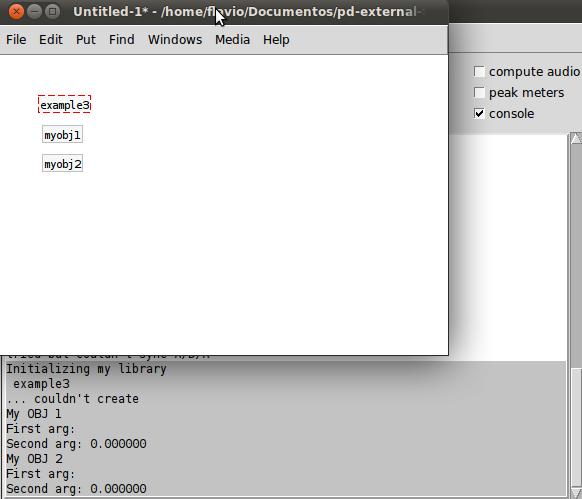
\includegraphics[width=0.7\textwidth]{example3}
	\caption{Nosso primeiro \external do PD. Ainda inútil.:-)}
\end{figure}


No caso da biblioteca, podemos ter um arquivo de help para cada \external. Esta
associação é feita pela função:

\vspace{1em}
\begin{lstlisting}
class_sethelpsymbol(myclass_class, gensym("my_class-help"));
\end{lstlisting}

Um objeto pode ainda ter outros nomes ou alias. Para definir isto podemo utilizar a função class\_addcreator. Veja o exemplo:

\vspace{1em}
\begin{lstlisting}
class_addcreator((t_newmethod)medusa_new, gensym("med"), 0);
\end{lstlisting}

\section{Variáveis globais}

Você pode usar uma variável global para armazenar dados pelos seus \externals.
Esta variável será visível para todas as intâncias do \external e todas podem
alterar seu valor. Isto pode ser útil ou um desastre. (Veja o exemplo16).

\vspace{1em}
\begin{lstlisting}
int count = 0;

void * example16_new(void) {
    t_example16 *x = (t_example16 *) pd_new(example16_class);
    post("Counter value: %d",count);
    count++;
    return (void *) x;
}
\end{lstlisting}

\begin{figure}[h!]
	\centering
	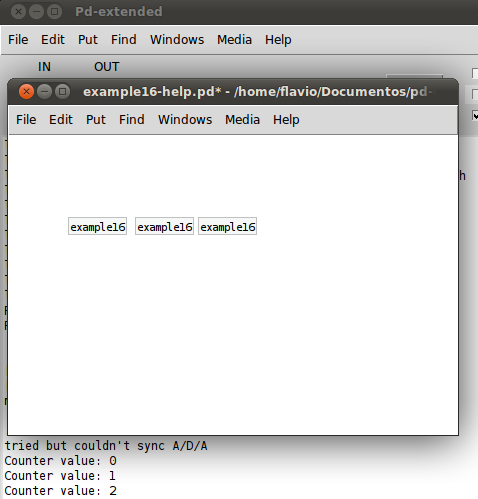
\includegraphics[width=0.7\textwidth]{example16}
	\caption{Repare no output da janela principal.}
\end{figure}

Caso isto não seja desejável, o ideal é colocar suas variáveis dentro da
struct do objeto. Assim cada instância terá seu próprio contador.

\vspace{1em}
\begin{lstlisting}
static t_class *example_class;

typedef struct _example {
    t_object x_obj;
    t_int counter;
} t_example;

void * example_new(void) {
    t_example *x = (t_example *) pd_new(example_class);
    post("Counter value: %d",x->counter);
    counter++;
    return (void *) x;
}

\end{lstlisting}


% ----------------------------------------------------------------------------
% OS TIPOS DE DADOS DO PD
% ----------------------------------------------------------------------------

\chapter{Os tipos de dados do PD}

Você pode usar os tipos de dados padrões do C, como int, float ou char. O
difícil é entender o que chamamos de tipos de dados padrões do C já que estes
tipos podem variar de acordo com o sistema operacional, compilador e outras
coisas. Por isto, para o external possa se comportar da mesma maneira em
qualquer sistema, é bastante recomendado que usemos os tipos do pure data.

Os tipos do pure data nada mais são que um


% ----------------------------------------------------------------------------
% CONSTRUTOR E DESTRUTOR
% ----------------------------------------------------------------------------

\chapter{Construtor e destrutor}

O Construtor de um objeto pode receber parâmetros. Estes parâmetros são
ilustrados abaixo.

\begin{figure}[h!]
	\centering
	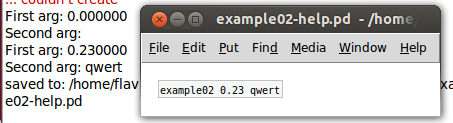
\includegraphics[width=0.7\textwidth]{example2}
	\caption{External recebendo parâmetros. Note a tela de saída no fundo da imagem.}
\end{figure}

\section{Construtor}

Parâmetros de inicialização no construtor podem permitir que inicializemos o
external com determinados valores. Isto é feito definindo os parâmetros no
métodos class\_new() quanto na definição da função construtora. (Veja o
exemplo02).

\begin{lstlisting}
// Constructos of the class
void * example2_new(t_symbol * arg1, t_floatarg arg2) {
    t_example2 *x = (t_example2 *) pd_new(example2_class);
    post("First arg: %s", arg1->s_name);
    post("Second arg: %f", arg2);
    return (void *) x;
}

void example2_setup(void) {
    example2_class = class_new(gensym("example2"),
            (t_newmethod) example2_new, // Constructor
            0,
            sizeof (t_example2),
	    CLASS_NOINLET,
            A_DEFFLOAT, // First Constructor parameter
            A_DEFSYMBOL, // Second Constructor parameter
            0);
}
\end{lstlisting}

Notem que os parâmetros são definidos com um tipo e são recebidos com outro.
Como explicado na seção \ref{sec:mensagens}, todos os dados que não
correspondem a sinais de áudio são transmitidos como mensagens, compostas de
átomos. Para ver os tipos de átomo que podem ser utilizados na passagem de
parâmetros, veja a seção \ref{sec:atomos}.

Para aceitar qualquer tipo de átomo na passagem de um parâmetro específico,
utilize o tipo de átomo \texttt{A\_GIMME} (veja o exemplo09).

\begin{lstlisting}
// Constructor of the class
void * example9_new(t_symbol *s, int argc, t_atom * argv) {
   t_example9 *x = (t_example9 *) pd_new(example9_class);
   post("%d parameters received",argc);
   return (void *) x;
}

void example9_setup(void) {
   example9_class = class_new(gensym("example9"),
     (t_newmethod) example9_new, // Constructor
     (t_method) example9_destroy, // Destructor
     sizeof (t_example9),
     CLASS_NOINLET,
     A_GIMME, // Allows various parameters
     0); // LAST argument is ALWAYS zero
}
\end{lstlisting}

Quando utilizamos o tipo de átomo \texttt{A\_GIMME} o método construtor
funciona como uma função \texttt{main()} em C: ela recebe os parâmetros
\texttt{argc}, que indica o número de átomos na lista, e \texttt{*argv}, que
aponta para a lista de átomos de fato. Veja o exemplo na figura
\ref{fig:construtor-parametros}.

\begin{figure}[h!]
\centering
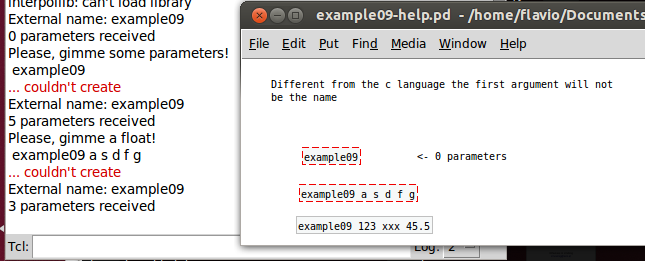
\includegraphics[width=0.7\textwidth]{example9}
\caption{Diferente da linguagem C, o primeiro parâmetro não é o nome do external.}
\label{fig:construtor-parametros}
\end{figure}

Note que o Pure Data não obriga que o usuário passe parâmetros para o objeto. É
como se todo construtor, independentemente de como ele está definido, aceitasse
sua instanciação vazia. Cabe ao programador verificar se os parâmetros
recebidos são em quantidade, tipo e valor esperado e, caso não seja, abortar a
construção do objeto e não retornar sua instância.

\section{Destrutor}

O destrutor de uma classe permite liberar alguma memória eventualmente alocada
pelo construtor ou por outras funções do \external (veja o exemplo 07).

\begin{lstlisting}
// Destroy the object
void example9_destroy(t_example9 *x) {
  post("You say good bye and I say hello");
}

void example9_setup(void) {
   example9_class = class_new(gensym("example9"),
     (t_newmethod) example9_new, // Constructor
     (t_method) example9_destroy, // Destructor
     sizeof (t_example9),
     CLASS_NOINLET,
     A_GIMME, // Allows various parameters
     0); // LAST argument is ALWAYS zero
}
\end{lstlisting}

A liberação da memória pode ser feita utilizando a função \texttt{freebytes()}
definida na API do Pure Data.

\begin{lstlisting}
void freebytes(void *x, size_t nbytes)
\end{lstlisting}


\section{Inlets e Outlets}


\begin{frame}{Inlets e outlets}
\begin{figure}[ht!]
\centering
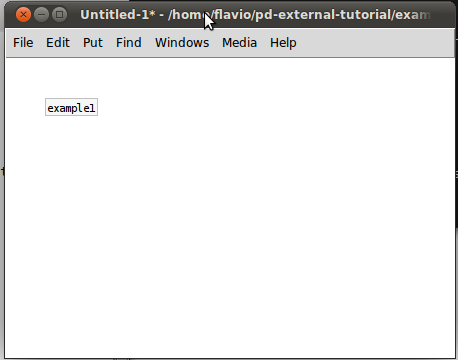
\includegraphics[height=0.6\textheight]{example1}
\caption{Para que serve isso!?}
\end{figure}
\end{frame}


\begin{frame}{Inlets passivos (1/3)}
\begin{figure}[h!]
\centering
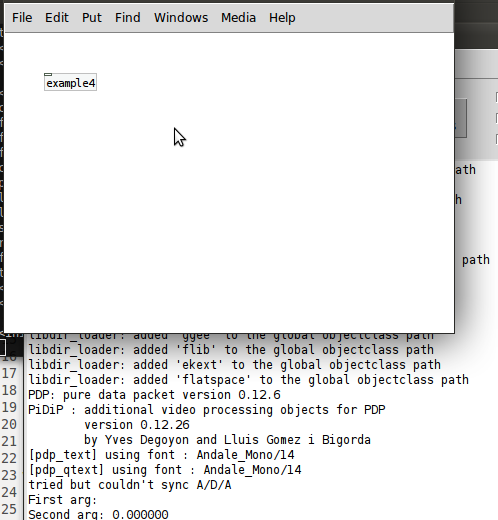
\includegraphics[height=0.8\textheight]{example4}
\label{fig:inlet-passivo}
\end{figure}
\end{frame}


\begin{frame}[fragile]{Inlets passivos (2/3)}
\begin{lstlisting}
static t_class *example4_class;

typedef struct _example4 {
  t_object x_obj;
  t_float my_float;
} t_example4;

// Constructor of the class
void *example4_new(t_symbol *arg1, t_floatarg arg2) {
  t_example4 *x = (t_example4*)pd_new(example4_class);
  post("First arg: %s", arg1->s_name);
  post("Second arg: %f", arg2);
  floatinlet_new(&x->x_obj, &x->my_float);
  return (void *) x;
}
\end{lstlisting}
\end{frame}


\begin{frame}{Inlets passivos (3/3)}
As funções para criar inlets passivos dos tipos mais comuns são:
\begin{itemize}
\item \texttt{floatinlet\_new(t\_object *owner, t\_float *fp)}
\item \texttt{symbolinlet\_new(t\_object *owner, t\_symbol **sp)}
\item \texttt{pointerinlet\_new(t\_object *owner, t\_gpointer *gp)}
\end{itemize}
\end{frame}


\begin{frame}{Inlets ativos (1/2)}
\begin{figure}[h!]
\centering
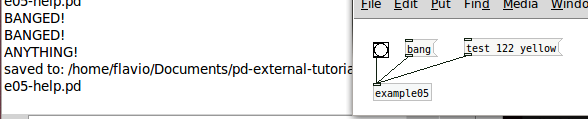
\includegraphics[width=0.7\textwidth]{example5}
\caption{Inlets ativos.}
\label{fig:inlet-ativo}
\end{figure}
\end{frame}


\begin{frame}[fragile]{Inlets ativos (2/2)}
\begin{lstlisting}[language=C]
// inlet-methods receive the object as first argument.
void example5_bang(t_example5 *x) { 
  post("BANGED!");
  post("My_float value: %f",x->my_float);
}

void example5_anything(t_example5 *x, t_symbol *s, int argc, t_atom *argv){
  post("ANYTHING!");
}

void example5_setup(void) {
  example5_class = class_new(gensym("example5"),
    (t_newmethod) example5_new, // Constructor
    0,  sizeof (t_example5), CLASS_DEFAULT,
    0); // LAST argument is ALWAYS zero
  class_addbang(example5_class, example5_bang);
  class_addanything(example5_class, example5_anything);
}
\end{lstlisting}
\end{frame}

\begin{frame}{Tratamento de mensagens (1/4)}
\begin{figure}[h!]
\centering
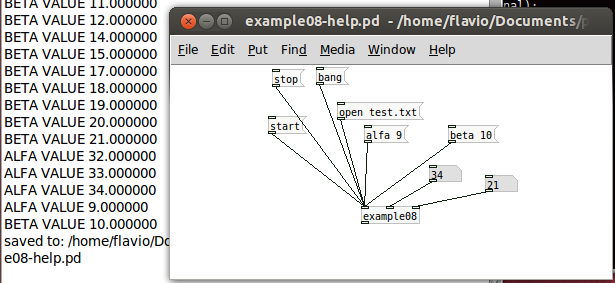
\includegraphics[width=0.7\textwidth]{example8}
\label{fig:inlet-ativo}
\end{figure}
\end{frame}

\begin{frame}[fragile]{Tratamento de mensagens (2/4)}
\lstinputlisting[name=Exemplo 08,linerange=47-61]{../examples/src/example08.c}
\end{frame}


\begin{frame}[fragile]{Tratamento de mensagens (3/4)}
\lstinputlisting[name=Exemplo 08,linerange=17-25,firstnumber=last]{../examples/src/example08.c}
\end{frame}


\begin{frame}[fragile]{Tratamento de mensagens (4/4)}
\lstinputlisting[name=Exemplo 08,linerange=27-45,firstnumber=last]{../examples/src/example08.c}
\end{frame}


\begin{frame}{Outlets (1/4)}
\begin{figure}[h!]
\centering
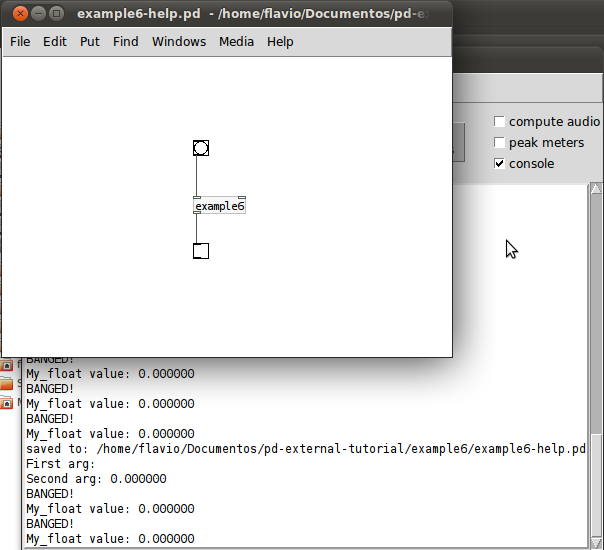
\includegraphics[width=0.7\textwidth]{example6}
\caption{Um external bem útil que recebe um bang e envia um bang.}
\label{fig:outlet-bang}
\end{figure}
\end{frame}


\begin{frame}{Outlets (2/4)}
\lstinputlisting[name=Exemplo 06,linerange=35-45]{../examples/src/example06.c}
\end{frame}


\begin{frame}{Outlets (3/4)}
\lstinputlisting[name=Exemplo 06,linerange=23-33,firstnumber=last]{../examples/src/example06.c}
\end{frame}


\begin{frame}{Outlets (4/4)}
\lstinputlisting[name=Exemplo 06,linerange=6-21,firstnumber=last]{../examples/src/example06.c}
\end{frame}


\section{Conclusão}

\begin{frame}{Referências}
\begin{itemize}
\item Repositório oficial de externals do Pure Data\footnote{http://pure-data.svn.sourceforge.net/viewvc/pure-data/trunk/externals}.
\item Tutorial do IOHannes\footnote{http://iem.at/pd/externals-HOWTO/pd-externals-HOWTO.pdf}.
\item Código fonte do Pure Data\footnote{http://pure-data.git.sourceforge.net/}.
\end{itemize}
\end{frame}


\begin{frame}{Dúvidas?}
{Obrigado!}
\texttt{http://www.ime.usp.br/$\sim$fls}

\texttt{https://github.com/flschiavoni/pd-external-tutorial}

\texttt{http://compmus.ime.usp.br/}
\end{frame}



\end{document}
